\tikzset{every picture/.style={line width=0.75pt}} %set default line width to 0.75pt        

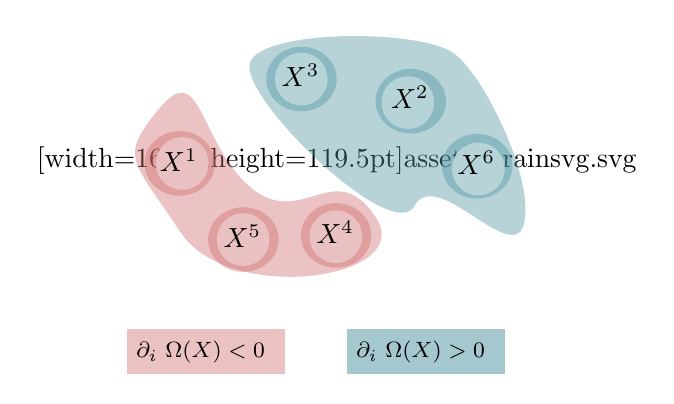
\begin{tikzpicture}[x=0.75pt,y=0.75pt,yscale=-1,xscale=1]
%uncomment if require: \path (0,293); %set diagram left start at 0, and has height of 293

%Image [id:dp7777581298700516] 
\draw (151.33,97) node  {\includesvg[width=163pt,height=119.5pt]{assets/brainsvg.svg}};
%Shape: Polygon Curved [id:ds18393926555266948] 
\draw  [draw opacity=0][fill={rgb, 255:red, 206; green, 106; blue, 107 }  ,fill opacity=0.4 ] (66,71.67) .. controls (86.13,47.55) and (84.8,88.22) .. (109.47,109.55) .. controls (134.13,130.88) and (150.13,94.22) .. (170.13,124.22) .. controls (190.13,154.22) and (99.47,166.88) .. (76.13,131.55) .. controls (52.8,96.22) and (45.87,95.78) .. (66,71.67) -- cycle ;
%Shape: Polygon Curved [id:ds5930593507912458] 
\draw  [draw opacity=0][fill={rgb, 255:red, 74; green, 145; blue, 158 }  ,fill opacity=0.4 ] (109.47,50.08) .. controls (114.13,33.42) and (192.8,33.42) .. (208.13,45.55) .. controls (223.47,57.68) and (246.8,106.88) .. (241.47,127.55) .. controls (236.13,148.22) and (199.47,99.42) .. (188.8,118.75) .. controls (184.88,125.85) and (172.5,120.72) .. (158.64,110.55) .. controls (134.77,93.04) and (106.51,60.63) .. (109.47,50.08) -- cycle ;
%Shape: Circle [id:dp1678818803252513] 
\draw  [draw opacity=0][fill={rgb, 255:red, 255; green, 255; blue, 255 }  ,fill opacity=1 ] (64.21,98.63) .. controls (64.05,91.62) and (69.6,85.8) .. (76.62,85.64) .. controls (83.63,85.47) and (89.45,91.03) .. (89.61,98.04) .. controls (89.77,105.06) and (84.22,110.88) .. (77.2,111.04) .. controls (70.19,111.2) and (64.37,105.65) .. (64.21,98.63) -- cycle ;
%Shape: Circle [id:dp6869227528745232] 
\draw  [draw opacity=0][fill={rgb, 255:red, 255; green, 255; blue, 255 }  ,fill opacity=1 ] (138.21,133.97) .. controls (138.05,126.95) and (143.6,121.13) .. (150.62,120.97) .. controls (157.63,120.81) and (163.45,126.36) .. (163.61,133.38) .. controls (163.77,140.39) and (158.22,146.21) .. (151.2,146.37) .. controls (144.19,146.54) and (138.37,140.98) .. (138.21,133.97) -- cycle ;
%Shape: Circle [id:dp5438595708004899] 
\draw  [draw opacity=0][fill={rgb, 255:red, 255; green, 255; blue, 255 }  ,fill opacity=1 ] (93.54,135.3) .. controls (93.38,128.29) and (98.93,122.47) .. (105.95,122.3) .. controls (112.96,122.14) and (118.78,127.7) .. (118.95,134.71) .. controls (119.11,141.73) and (113.55,147.55) .. (106.54,147.71) .. controls (99.52,147.87) and (93.7,142.32) .. (93.54,135.3) -- cycle ;
%Shape: Circle [id:dp6212121433012971] 
\draw  [draw opacity=0][fill={rgb, 255:red, 255; green, 255; blue, 255 }  ,fill opacity=1 ] (121.54,57.97) .. controls (121.38,50.95) and (126.93,45.13) .. (133.95,44.97) .. controls (140.96,44.81) and (146.78,50.36) .. (146.95,57.38) .. controls (147.11,64.39) and (141.55,70.21) .. (134.54,70.37) .. controls (127.52,70.54) and (121.7,64.98) .. (121.54,57.97) -- cycle ;
%Shape: Circle [id:dp7627341450544065] 
\draw  [draw opacity=0][fill={rgb, 255:red, 255; green, 255; blue, 255 }  ,fill opacity=1 ] (206.87,101.3) .. controls (206.71,94.29) and (212.27,88.47) .. (219.28,88.3) .. controls (226.3,88.14) and (232.12,93.7) .. (232.28,100.71) .. controls (232.44,107.73) and (226.89,113.55) .. (219.87,113.71) .. controls (212.86,113.87) and (207.04,108.32) .. (206.87,101.3) -- cycle ;
%Shape: Circle [id:dp1869737705120207] 
\draw  [draw opacity=0][fill={rgb, 255:red, 255; green, 255; blue, 255 }  ,fill opacity=1 ] (172.87,69.3) .. controls (172.71,62.29) and (178.27,56.47) .. (185.28,56.3) .. controls (192.3,56.14) and (198.12,61.7) .. (198.28,68.71) .. controls (198.44,75.73) and (192.89,81.55) .. (185.87,81.71) .. controls (178.86,81.87) and (173.04,76.32) .. (172.87,69.3) -- cycle ;

% Text Node
\draw  [draw opacity=0][fill={rgb, 255:red, 206; green, 106; blue, 107 }  ,fill opacity=0.41 ]  (151, 133) circle [x radius= 16.97, y radius= 15.56]   ;
\draw (140,124.4) node [anchor=north west][inner sep=0.75pt]    {$X^{4}$};
% Text Node
\draw  [draw opacity=0][fill={rgb, 255:red, 206; green, 106; blue, 107 }  ,fill opacity=0.41 ]  (75.67, 98.33) circle [x radius= 16.97, y radius= 15.56]   ;
\draw (64.67,89.73) node [anchor=north west][inner sep=0.75pt]    {$X^{1}$};
% Text Node
\draw  [draw opacity=0][fill={rgb, 255:red, 206; green, 106; blue, 107 }  ,fill opacity=0.41 ]  (106.33, 135) circle [x radius= 16.97, y radius= 15.56]   ;
\draw (95.33,126.4) node [anchor=north west][inner sep=0.75pt]    {$X^{5}$};
% Text Node
\draw  [draw opacity=0][fill={rgb, 255:red, 74; green, 145; blue, 158 }  ,fill opacity=0.4 ]  (134.33, 57.67) circle [x radius= 16.97, y radius= 15.56]   ;
\draw (123.33,49.07) node [anchor=north west][inner sep=0.75pt]    {$X^{3}$};
% Text Node
\draw  [draw opacity=0][fill={rgb, 255:red, 74; green, 145; blue, 158 }  ,fill opacity=0.4 ]  (187, 68.33) circle [x radius= 16.97, y radius= 15.56]   ;
\draw (176,59.73) node [anchor=north west][inner sep=0.75pt]    {$X^{2}$};
% Text Node
\draw  [draw opacity=0][fill={rgb, 255:red, 74; green, 145; blue, 158 }  ,fill opacity=0.4 ]  (219, 99.67) circle [x radius= 16.97, y radius= 15.56]   ;
\draw (208,91.07) node [anchor=north west][inner sep=0.75pt]    {$X^{6}$};
% Text Node
\draw  [draw opacity=0][fill={rgb, 255:red, 206; green, 106; blue, 107 }  ,fill opacity=0.41 ]  (50.33,178) -- (126.33,178) -- (126.33,200) -- (50.33,200) -- cycle  ;
\draw (53.33,182.4) node [anchor=north west][inner sep=0.75pt]  [font=\footnotesize]  {$\partial _{i} \ \Omega ( X) < 0$};
% Text Node
\draw  [draw opacity=0][fill={rgb, 255:red, 74; green, 145; blue, 158 }  ,fill opacity=0.5 ]  (156.33,178) -- (232.33,178) -- (232.33,200) -- (156.33,200) -- cycle  ;
\draw (159.33,182.4) node [anchor=north west][inner sep=0.75pt]  [font=\footnotesize]  {$\partial _{i} \ \Omega ( X)  >0$};


\end{tikzpicture}
